\section{Hasil}

\subsection{Verifikasi Implementasi}
\label{sec:verifikasi}

Seluruh 37 uji unit lolos (\Tabelref{tab:uji}). Uji fitness dan validasi memakai angka dari data asli. Contohnya, rute National Monument $\to$ Merdeka Square $\to$ Irian Jaya Liberation Monument untuk dua orang berbiaya Rp58.095 dengan durasi 1,45 jam. Rute ini dinyatakan VALID untuk anggaran Rp60.000 dan batas 2 jam, tetapi TIDAK VALID bila anggarannya Rp58.000 atau batas jamnya 1,4 jam.

\begin{table}[H]
\centering
\caption{Uji unit pada \texttt{tests/ga.test.ts}.}
\label{tab:uji}
\small
\begin{tabular}{@{}l c >{\raggedright\arraybackslash}p{9.6cm}@{}}
\toprule
\textbf{Kelompok} & \textbf{Uji} & \textbf{Yang diuji} \\
\midrule
Data & 4 & 201 atraksi, matriks dicari per nama, format CSV, penolakan data tidak sah \\
Fitness dan validasi & 10 & biaya, durasi, VALID/TIDAK VALID, rumus fitness, penalti, bonus minat, jadwal harian \\
Kromosom & 3 & dekode, penulisan ulang urutan, penyandian rute \\
Crossover & 3 & OX mereproduksi contoh Davis \cite{davis1985}, anak selalu permutasi sah, uniform/one-point \\
Mutasi & 4 & swap, insert, tambah (termasuk tambah-lokal), hapus, kromosom tetap sah \\
Seleksi & 2 & frekuensi menang turnamen dan roulette sesuai teori \\
Loop GA & 8 & greedy seeding selalu valid, elitisme tidak pernah menurunkan fitness terbaik, determinisme seed, top-5 berbeda, stagnasi \\
Pembanding & 3 & greedy menghasilkan rute valid, pencarian acak memakai jumlah evaluasi yang sama \\
\midrule
\textbf{Total} & \textbf{37} & semua lolos \\
\bottomrule
\end{tabular}
\end{table}

Uji elitisme disertai uji pembanding: tanpa elitisme (seleksi roulette, elit 0), fitness terbaik terbukti bisa turun antargenerasi. Dengan begitu, lolosnya uji elitisme memang bermakna.

\subsection{Contoh Rekomendasi}

\Gambarref{fig:hasil} memperlihatkan hasil untuk skenario 1 dengan minat museum (bobot 1) dan sejarah (bobot 0,5), seed 42. GA selesai 200 generasi (19.700 evaluasi) dalam 0,36 detik. Kelima rencana VALID, hampir menghabiskan anggaran, dan jadwalnya muat dalam 5 hari (\Tabelref{tab:top5}).

\begin{figure}[H]
\centering
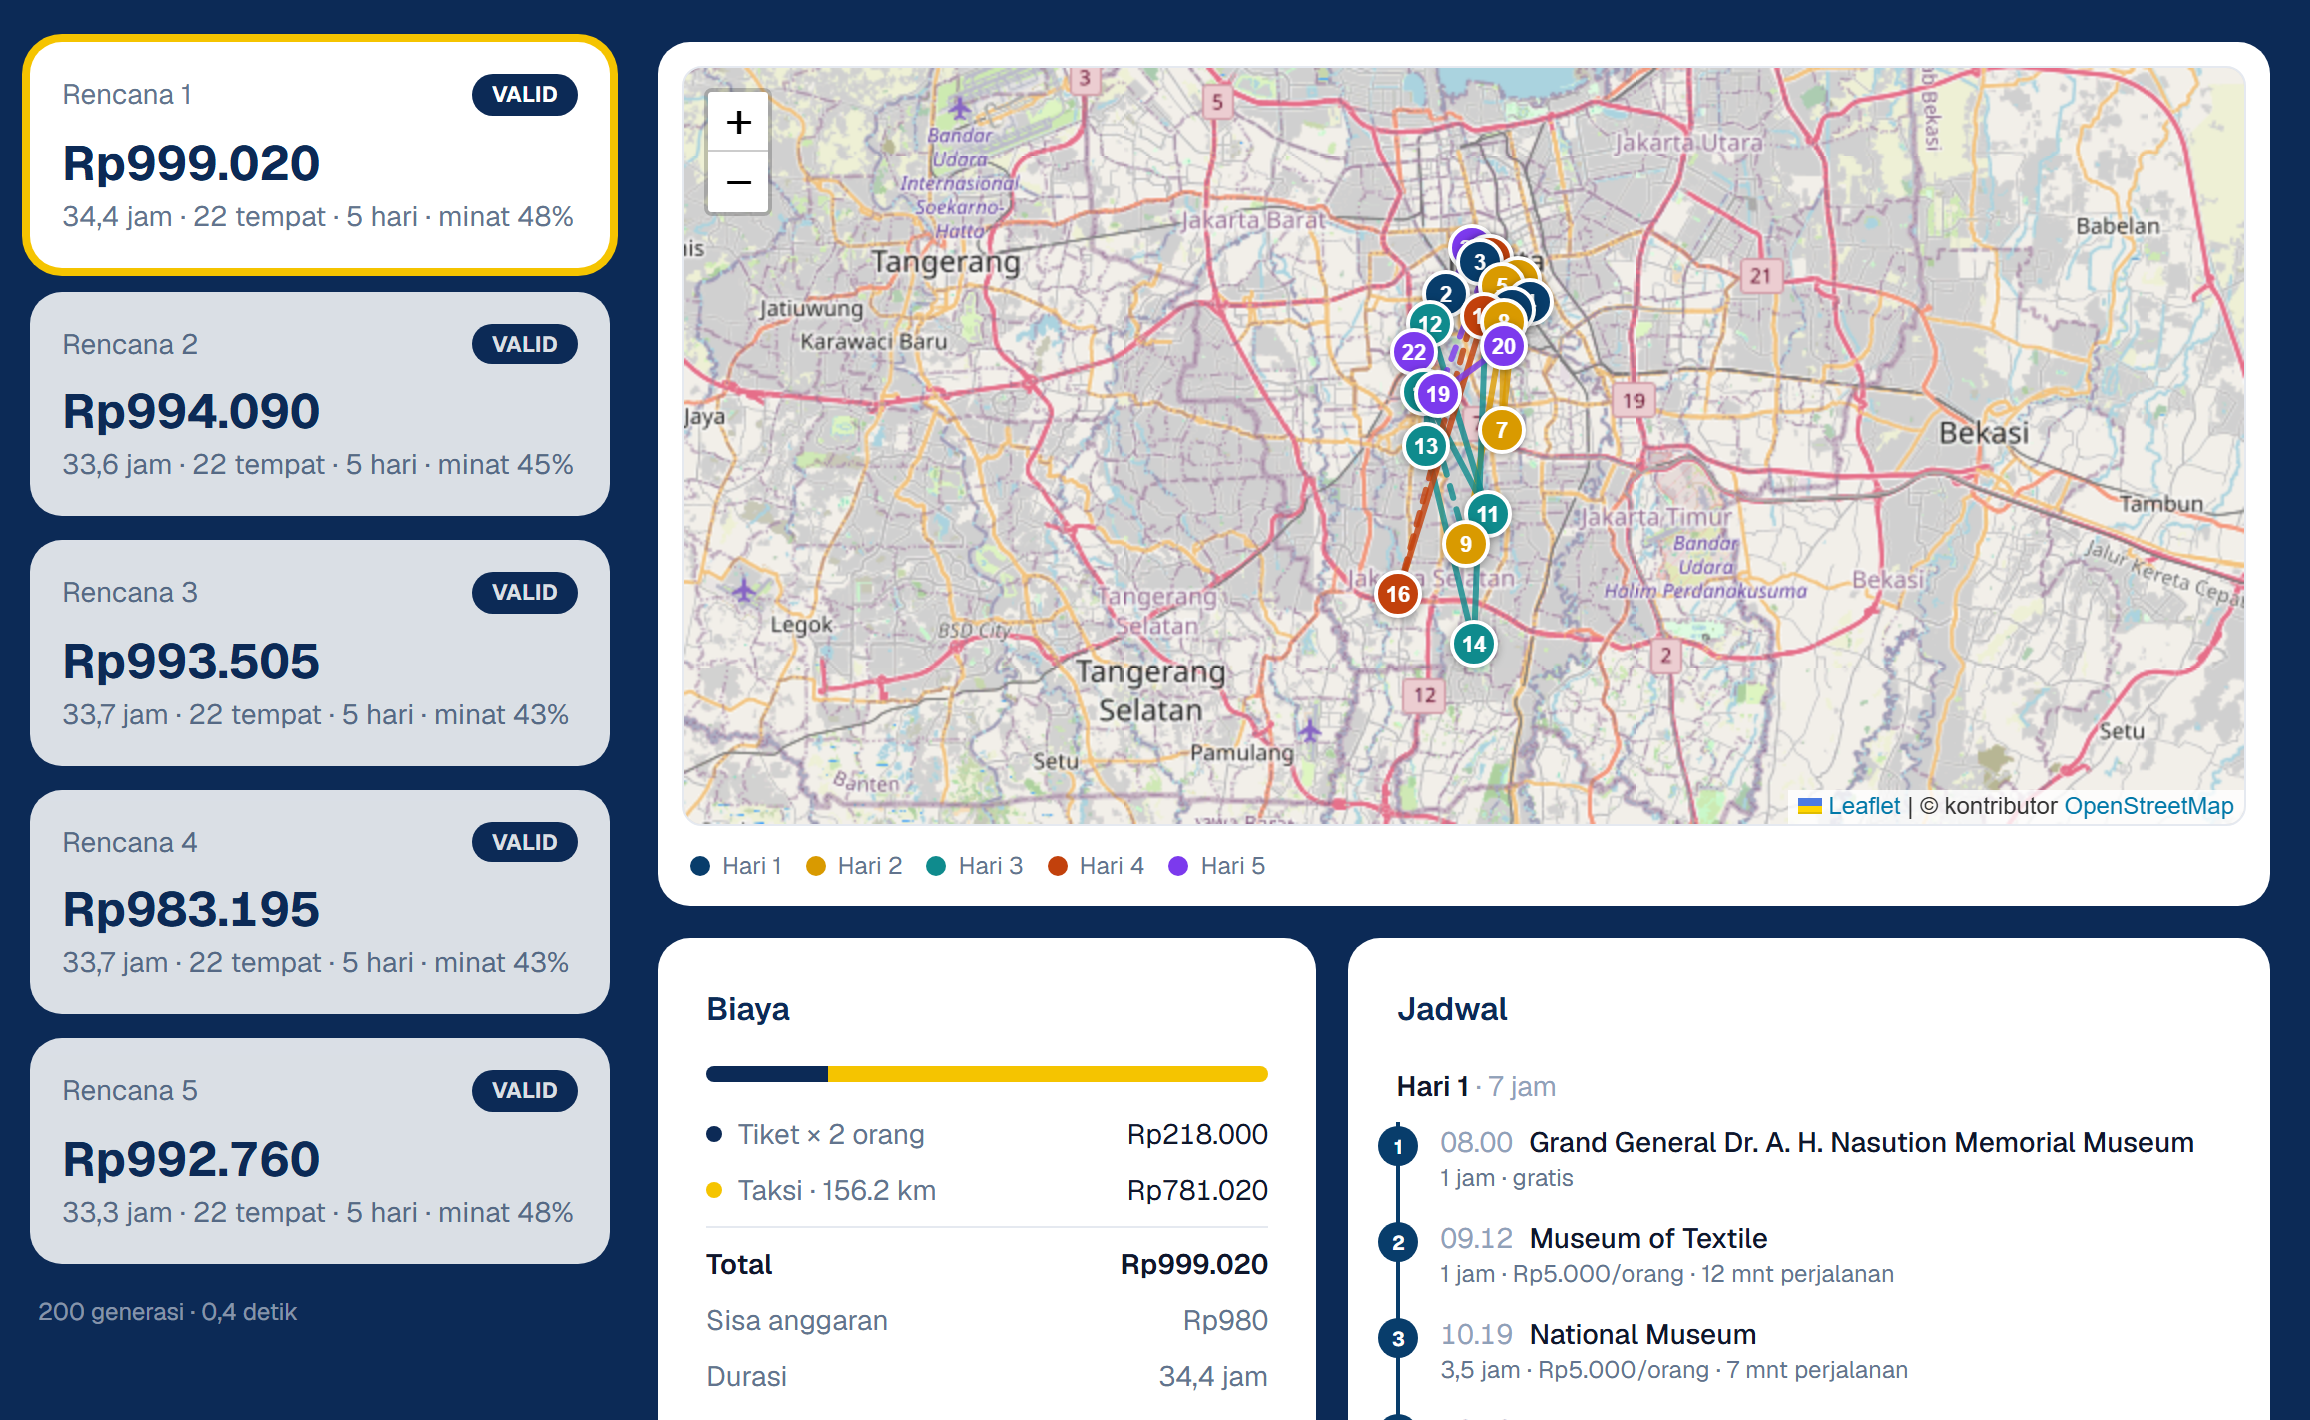
\includegraphics[width=\linewidth]{gambar/hasil-ringkas.png}
\caption{Halaman hasil aplikasi: lima rencana terbaik, peta rute berurutan (warna = hari), rincian biaya, dan jadwal harian.}
\label{fig:hasil}
\end{figure}

\begin{table}[H]
\centering
\caption{Lima rencana terbaik (Rp1.000.000; 5 hari $\times$ 7 jam; 2 orang; minat museum dan sejarah).}
\label{tab:top5}
\small
\begin{tabular}{@{}c r r c c c c c@{}}
\toprule
\textbf{Rencana} & \textbf{Biaya} & \textbf{Sisa} & \textbf{Durasi} & \textbf{Tempat} & \textbf{Minat} & \textbf{Fitness} & \textbf{Status} \\
\midrule
1 & Rp999.020 & Rp980    & 34,4 jam & 22 & 48\% & \textbf{50,73} & VALID \\
2 & Rp994.090 & Rp5.910  & 33,6 jam & 22 & 45\% & 26,49 & VALID \\
3 & Rp993.505 & Rp6.495  & 33,7 jam & 22 & 43\% & 26,01 & VALID \\
4 & Rp983.195 & Rp16.805 & 33,7 jam & 22 & 43\% & 22,54 & VALID \\
5 & Rp992.760 & Rp7.240  & 33,3 jam & 22 & 48\% & 22,46 & VALID \\
\bottomrule
\end{tabular}
\end{table}

Rencana 1 terdiri dari 29,25 jam kunjungan dan 5,12 jam perjalanan (156,2 km). Biayanya Rp218.000 untuk tiket dua orang dan Rp781.020 untuk taksi. Jadwalnya terbagi menjadi 4, 5, 6, 3, dan 4 destinasi per hari, masing-masing 6,7--7,0 jam. Hari pertama berisi empat destinasi bertema museum yang saling berdekatan: Grand General Dr.\ A.\ H.\ Nasution Memorial Museum, Museum of Textile (12 menit perjalanan), National Museum (7 menit), dan Jakarta Planetarium (9 menit).

\subsection{Konvergensi}

Fitness terbaik naik dari 11,77 pada generasi awal menjadi 50,73 pada generasi 200 (\Gambarref{fig:konvergensi}), atau 4,3 kali. Kurva terbaik tidak pernah turun karena elitisme dan naik bertahap setiap kali GA menemukan kombinasi yang lebih seimbang. Rata-rata fitness populasi naik dari 1,42 menjadi 6,10, sedangkan porsi individu valid naik dari 44\% menjadi 58\%.

\begin{figure}[H]
\centering
\begin{tikzpicture}
\begin{axis}[
  width=0.9\linewidth, height=6.2cm, xmin=0, xmax=200, ymin=0, ymax=60,
  xlabel={Generasi}, ylabel={Fitness}, axis y line*=left,
  legend style={at={(0.02,0.98)}, anchor=north west, font=\footnotesize, draw=none, fill=white, fill opacity=0.85, text opacity=1},
  tick label style={font=\footnotesize}, label style={font=\small}, grid=major, grid style={gray!15}]
\addplot[ugmnavy, very thick, const plot] table[x=gen, y=terbaik]{data/konvergensi.dat};
\addlegendentry{Fitness terbaik}
\addplot[ugmgold!85!black, thick] table[x=gen, y=ratarata]{data/konvergensi.dat};
\addlegendentry{Fitness rata-rata}
\addlegendimage{abu, dashed}
\addlegendentry{Individu valid (\%)}
\end{axis}
\begin{axis}[
  width=0.9\linewidth, height=6.2cm, xmin=0, xmax=200, ymin=0, ymax=100,
  axis y line*=right, axis x line=none, ylabel={Individu valid (\%)},
  tick label style={font=\footnotesize}, label style={font=\small}]
\addplot[abu, dashed] table[x=gen, y=valid]{data/konvergensi.dat};
\end{axis}
\end{tikzpicture}
\caption{Fitness terbaik dan rata-rata per generasi serta porsi individu valid (skenario pada \Tabelref{tab:top5}).}
\label{fig:konvergensi}
\end{figure}

\Gambarref{fig:sebaran} menunjukkan error biaya dan error durasi tiap individu pada populasi akhir. Keduanya saling tarik-menarik: rencana yang tepat waktu bisa boros biaya, dan sebaliknya. Individu yang paling seimbang hanya meleset 0,64 jam dan Rp980 dari target.

\begin{figure}[H]
\centering
\begin{tikzpicture}
\begin{axis}[
  width=0.9\linewidth, height=6cm, xmin=0, xmax=7, ymin=0, ymax=220,
  xlabel={$|$error durasi$|$ (jam)}, ylabel={$|$error biaya$|$ (Rp ribu)},
  legend style={at={(0.98,0.98)}, anchor=north east, font=\footnotesize, draw=none, fill=white, fill opacity=0.85, text opacity=1},
  tick label style={font=\footnotesize}, label style={font=\small}, grid=major, grid style={gray!15}]
\addplot[only marks, mark=*, mark size=1.7pt, ugmnavy] table[x=jam, y=biaya]{data/sebaran-valid.dat};
\addlegendentry{Valid}
\addplot[only marks, mark=*, mark size=1.4pt, abu!70] table[x=jam, y=biaya]{data/sebaran-tidak.dat};
\addlegendentry{Tidak valid}
\addplot[only marks, mark=*, mark size=4pt, ugmgold, draw=ugmnavy] table[x=jam, y=biaya]{data/sebaran-seimbang.dat}
  node[pos=0, anchor=west, font=\footnotesize\bfseries, ugmnavy, xshift=6pt, yshift=12pt, fill=white, inner sep=1pt] {paling seimbang};
\addlegendentry{Paling seimbang}
\end{axis}
\end{tikzpicture}
\caption{Error biaya terhadap error durasi pada populasi akhir. Sumbu dipotong pada persentil 90 agar klaster utama terlihat.}
\label{fig:sebaran}
\end{figure}

\subsection{Perbandingan dengan Metode Lain}

\Tabelref{tab:banding} dan \Gambarref{fig:banding} merangkum 20 run untuk setiap metode dan skenario. Semua metode selalu menghasilkan rencana valid, tetapi kualitasnya sangat berbeda. Fitness rata-rata GA \textbf{5,9; 3,8; dan 4,5 kali} pembanding terbaik pada skenario 1, 2, dan 3.

\begin{table}[H]
\centering
\caption{Perbandingan metode (rata-rata 20 seed). Pencarian acak memakai jumlah evaluasi yang sama dengan GA.}
\label{tab:banding}
\small
\setlength{\tabcolsep}{4.5pt}
\begin{tabular}{@{}c l r r r r r@{}}
\toprule
\textbf{Sk.} & \textbf{Metode} & \textbf{Fitness} & \textbf{Terbaik} & \textbf{Biaya} & \textbf{Durasi} & \textbf{Waktu} \\
\midrule
\multirow{4}{*}{1} & \textbf{Algoritma Genetika} & \textbf{22,62} $\pm$ 4,88 & \textbf{31,13} & Rp996.297 & 33,9 jam & 609 ms \\
 & Greedy termurah dulu & 1,09 $\pm$ 0,00 & 1,09 & Rp216.345 & 30,6 jam & $<$1 ms \\
 & Greedy terdekat dulu & 3,77 $\pm$ 2,18 & 9,46 & Rp847.777 & 28,7 jam & $<$1 ms \\
 & Pencarian acak & 3,82 $\pm$ 0,55 & 4,93 & Rp972.738 & 27,4 jam & 997 ms \\
\midrule
\multirow{4}{*}{2} & \textbf{Algoritma Genetika} & \textbf{82,62} $\pm$ 20,84 & \textbf{126,99} & Rp2.994.914 & 29,7 jam & 590 ms \\
 & Greedy termurah dulu & 1,50 $\pm$ 0,00 & 1,50 & Rp203.970 & 29,0 jam & $<$1 ms \\
 & Greedy terdekat dulu & 2,62 $\pm$ 1,57 & 6,88 & Rp1.173.908 & 26,9 jam & $<$1 ms \\
 & Pencarian acak & 21,64 $\pm$ 7,78 & 41,44 & Rp2.941.828 & 28,8 jam & 1.038 ms \\
\midrule
\multirow{4}{*}{3} & \textbf{Algoritma Genetika} & \textbf{76,25} $\pm$ 25,58 & \textbf{122,68} & Rp498.033 & 13,8 jam & 396 ms \\
 & Greedy termurah dulu & 1,80 $\pm$ 0,00 & 1,80 & Rp163.510 & 13,0 jam & $<$1 ms \\
 & Greedy terdekat dulu & 4,41 $\pm$ 2,31 & 9,92 & Rp397.167 & 11,2 jam & $<$1 ms \\
 & Pencarian acak & 16,95 $\pm$ 5,87 & 36,85 & Rp484.135 & 13,2 jam & 1.222 ms \\
\bottomrule
\end{tabular}
\end{table}

\begin{figure}[H]
\centering
\begin{tikzpicture}
\begin{axis}[
  ybar, bar width=12pt, width=0.9\linewidth, height=6cm, ymin=0, ymax=95,
  symbolic x coords={Skenario 1, Skenario 2, Skenario 3}, xtick=data, xtick style={draw=none}, enlarge x limits=0.22,
  ylabel={Fitness rata-rata}, nodes near coords style={font=\scriptsize, /pgf/number format/use comma},
  legend style={at={(0.5,-0.14)}, anchor=north, legend columns=4, font=\footnotesize, draw=none, /tikz/every even column/.append style={column sep=8pt}},
  legend image code/.code={\draw[#1, draw=none] (0cm,-0.08cm) rectangle (0.3cm,0.12cm);},
  tick label style={font=\footnotesize}, label style={font=\small}, ymajorgrids, grid style={gray!15}]
\addplot[fill=ugmnavy, draw=none, nodes near coords] coordinates {(Skenario 1,22.62) (Skenario 2,82.62) (Skenario 3,76.25)};
\addplot[fill=ugmgold, draw=none] coordinates {(Skenario 1,1.09) (Skenario 2,1.50) (Skenario 3,1.80)};
\addplot[fill=abu, draw=none] coordinates {(Skenario 1,3.77) (Skenario 2,2.62) (Skenario 3,4.41)};
\addplot[fill=gray!35, draw=none, nodes near coords] coordinates {(Skenario 1,3.82) (Skenario 2,21.64) (Skenario 3,16.95)};
\legend{Algoritma Genetika, Greedy termurah, Greedy terdekat, Pencarian acak}
\end{axis}
\end{tikzpicture}
\caption{Fitness rata-rata setiap metode (20 seed per skenario).}
\label{fig:banding}
\end{figure}

\subsection{Sensitivitas Parameter}

\Tabelref{tab:sensitivitas} dan \Gambarref{fig:sensitivitas} memperlihatkan pengaruh tiap parameter pada skenario 1 (10 seed per nilai). Semua run menghasilkan rencana valid.

\begin{table}[H]
\centering
\caption{Fitness rata-rata $\pm$ simpangan baku dan waktu per run. Tebal = nilai bawaan.}
\label{tab:sensitivitas}
\small
\begin{tabular}{@{}l c c c c@{}}
\toprule
\textbf{Ukuran populasi} & 25 & 50 & \textbf{100} & 200 \\
\midrule
Fitness & 18,04 $\pm$ 9,12 & 20,08 $\pm$ 6,94 & \textbf{21,54} $\pm$ 5,26 & 24,53 $\pm$ 4,32 \\
Waktu & 179 ms & 412 ms & 609 ms & 1.376 ms \\
\midrule
\textbf{Peluang mutasi} & 0,01 & \textbf{0,05} & 0,1 & 0,2 \\
\midrule
Fitness & 20,77 $\pm$ 12,66 & \textbf{21,54} $\pm$ 5,26 & 22,58 $\pm$ 9,66 & 14,86 $\pm$ 4,17 \\
Waktu & 409 ms & 609 ms & 759 ms & 883 ms \\
\midrule
\textbf{Peluang crossover} & 0,4 & 0,6 & \textbf{0,8} & 0,95 \\
\midrule
Fitness & 24,23 $\pm$ 6,56 & 26,55 $\pm$ 8,90 & \textbf{21,54} $\pm$ 5,26 & 23,57 $\pm$ 5,71 \\
Waktu & 446 ms & 406 ms & 480 ms & 458 ms \\
\bottomrule
\end{tabular}
\end{table}

\begin{figure}[H]
\centering
\pgfplotsset{sens/.style={width=5.4cm, height=4.2cm, ymin=0, ymax=40, symbolic x coords={a,b,c,d}, xtick=data,
  tick label style={font=\scriptsize}, label style={font=\footnotesize}, title style={font=\footnotesize\bfseries}, ymajorgrids, grid style={gray!15}}}
\begin{tikzpicture}
\begin{axis}[sens, title={Ukuran populasi}, ylabel={Fitness}, xticklabels={25, 50, 100, 200}]
\addplot[ugmnavy, thick, mark=*, error bars/.cd, y dir=both, y explicit] coordinates {(a,18.04) +- (0,9.12) (b,20.08) +- (0,6.94) (c,21.54) +- (0,5.26) (d,24.53) +- (0,4.32)};
\end{axis}
\end{tikzpicture}\hfill
\begin{tikzpicture}
\begin{axis}[sens, title={Peluang mutasi}, xticklabels={0{,}01, 0{,}05, 0{,}1, 0{,}2}]
\addplot[ugmnavy, thick, mark=*, error bars/.cd, y dir=both, y explicit] coordinates {(a,20.77) +- (0,12.66) (b,21.54) +- (0,5.26) (c,22.58) +- (0,9.66) (d,14.86) +- (0,4.17)};
\end{axis}
\end{tikzpicture}\hfill
\begin{tikzpicture}
\begin{axis}[sens, title={Peluang crossover}, xticklabels={0{,}4, 0{,}6, 0{,}8, 0{,}95}]
\addplot[ugmnavy, thick, mark=*, error bars/.cd, y dir=both, y explicit] coordinates {(a,24.23) +- (0,6.56) (b,26.55) +- (0,8.90) (c,21.54) +- (0,5.26) (d,23.57) +- (0,5.71)};
\end{axis}
\end{tikzpicture}
\caption{Fitness rata-rata $\pm$ simpangan baku terhadap nilai parameter (skenario 1, 10 seed).}
\label{fig:sensitivitas}
\end{figure}
